\chapter{A practical take at machine learning}
\section{Modern problems}

Machine learning is based on advanced algorithms and complex data structures, performing calculations on training and validation datasets provided by the user, aswell as data received during their regular operation.

Some of the most basic models are created via techniques such as linear and non-linear regression, logistics regression or linear discriminant analysis. They result in shallow machine learning models, which have relatively small computational complexity to evaluate results of a dataset in comparison to other models \cite{shallow}.

Few of the more soffisticated methods are for example decision trees, based on algorythmical tree logic \cite{tree}. Each of the tree layer corresponds to the best predictor available at a current state, causing branching to specific values or ranges of values. The result calculation is achieved via traversing the tree from the root to one of its ending leafs. 

The most advanced, yet at the same time most demanding in complexity and memory types of deep learning models such as deep neural networks, convolutional neural networks and recursive neural networks. They utilize structure consisting of one input layer, one or more hidden layers containing mathematical neurons, and one output layer. Each subsequent layer is connected to the previous one, either fully or partially, feeding the results of processing forward. Basic neural networks make neurons present in the same layer independent from one another. Each connection has its own weight, which is multiplied by the input from that connection, and sumed up with the results from other connections, to be passed forward to the activation function. This function decide whether a neuron should activate, and (in case of continuous range $\langle$0; 1$\rangle$) to what extent \cite{mit_neural}. An example of a network with a singular neuron was presented on figure \ref{fig:nn}.

\begin{figure}[!ht]
    \centering
    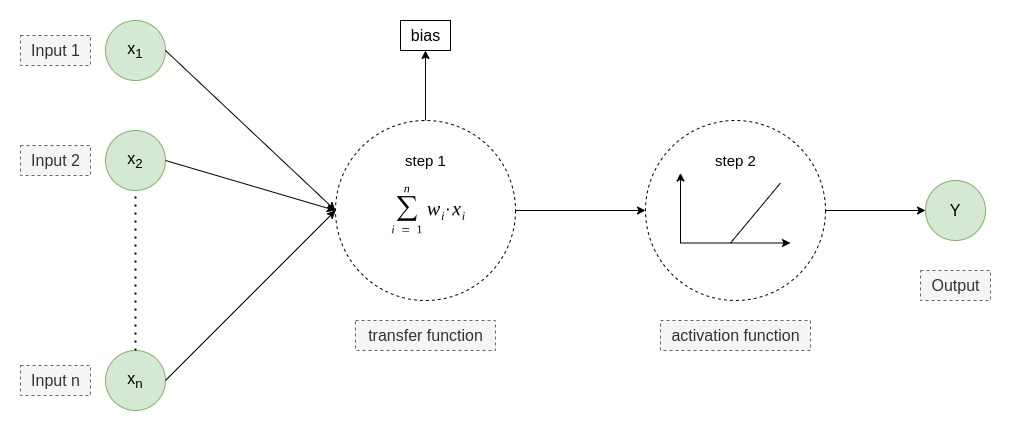
\includegraphics[width=150mm]{Rysunki/Rozdzial2/perceptron.jpg}
    \caption{Neuron blueprint -- Simplelearn.}
    \label{fig:nn}
\end{figure}

Extensive neural networks, such as CNN, require additional steps to preprocess the input data, such that it is acceptable by the network, like for example pooling. By analizing structures incorporated by each of the mentioned methods, following implementation challenges can be identified \cite{constrained}:

\newpage
\begin{itemize}
    \item [$\bullet$] Efficiency - it is tightly connected to the computational complexity of the used methods, aswell as the characteristics of used programming language and hardware platform. The desired effect would be to minimize the learning time of the model and propagation time from inputing the data to receiving a result. In most cases, minimalization of propagation time takes priority.
    
    \item [$\bullet$] Memory usage - this is a concern mainly when using platform with limited resources, such as microcontrolers and microcomputers, where current RAM and flash memory sizes (especially in embedded systems) can be very limited in comparison to regular computers or mobile platforms.
\end{itemize}

During development of machine learning technology, significant steps were taken into solving above mentioned problems, and fulfill everincreasing requirements of modern machine learning applications. Some of the ways this was achieved are algorithm optimization, selecting high frequency hardware platforms, utilizing paralel computing and using high performance compiled programming languages, especially those that support low level operations. 

\section{C++ as a solution to machine learning problems}

Among various languages and environments supporting machine learning, such as Python, C++, Java and Matlab, one of the special few is C++. It is an imperative language with strong typing, connecting low level functionalities for specific hardware architectures with high level programming. As such, it offers vast control over memory usage and optimization possibilities, like adjusting used types for the specific processing needs, contol over variable placing in memory (it is up to the developer to choose whether the data will be placed on stack or heap) and function call optimizations by inlining and tail recursion optimization. In contrary to scripting languages whose code is interpreted during execution, such as Python and Matlab language, C++ is a compiled language, which means that its code is converted into a binary executable adjusted to specific CPU architecture. This completely removes the overhead of interpreting the source code, as the conversion to CPU language is done only once, during the binary generation process. Additionally, this allows the compiler to perform various low level optimizations \cite{cpp_char}.

Parts of C++ mechanisms which find their root back in C language allow to use Assembly insets, further increasing the efficiency, at the cost of portability. Some platforms also offer API for hardware acceleration modules, such as eg. Neural Networks API - NNA - of Android, allowing for faster processing via specially designed hardware \cite{android_nna}.

\begin{figure}[!ht]
    \centering
    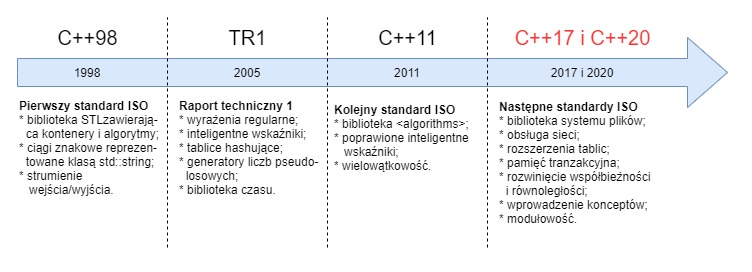
\includegraphics[width=150mm]{Rysunki/Rozdzial2/multithreading.jpg}
    \caption{Concurrency evolution in modern C++ - Modernes C++.}
    \label{fig:cpp_history}
\end{figure}

One of the major factors increasing efficiency of machine learning models is paralel processing. Availability of multithreading (added in C++11 standard and further developed, as presented in figure \ref{fig:cpp_history}) and compatibility with CUDA language and API \cite{cpp_cuda} allows C++ to perform many calculations simultaneously utilizing multiple cores of the CPU or delegating processing to one or many graphics cards (where the number of GPU processors vastly outnumbers CPU cores). Additional, although fairly obvious benefit of using this language is easy integration of the models with programs already made in the same language (which is often the case in embedded systems, IoT and computationally intensive software).

\section{The aim of creating libraries}

Due to the complexity of mechanisms that are part of machine learning, various experience of developers and the need for intense optimization, implementation of the machine learning methods is lengthy and expensive. Here programmers can seek for help in libraries created by corporations such as Google and big open-source communities. The libraries provide ready for use mechanisms (often created according to object oriented paradigm, via a set of classes), which are constantly updated and optimized by developers who use it in their daily work or passion projects. They offer a way to quickly create your own models, and often also allow to use already created pre-trained models on stock datasets. Important benefit of using existing libraries that are still supported is better stability, as parts of the library are implemented and tested by experienced developers, like in the case of TensorFlow library provided by Google.

Majority of libraries for machine learning, even in languages such as Python, are in fact made in C++, providing API for different languages. Sadly, not all libraries made in C++ offer suitable API to use in that same language, as a result, in most cases its use is convoluted and unnecessarily difficult. As a result, some of the libraries work with models created (even by this very same library) in different language, as is the case with TensorFlow lite. Common example is using Python to create a model graph or exporting model to ONNX format (Open Neural Network Exchange) \cite{cpp_onnx}. In this analysis, presented libraries offer the ability to create models in C++, without the need for other language. 